\iffalse

MIT License

Copyright (c) 2023 Aron Hardeman

Permission is hereby granted, free of charge, to any person obtaining a copy
of this software and associated documentation files (the "Software"), to deal
in the Software without restriction, including without limitation the rights
to use, copy, modify, merge, publish, distribute, sublicense, and/or sell
copies of the Software, and to permit persons to whom the Software is
furnished to do so, subject to the following conditions:

The above copyright notice and this permission notice shall be included in all
copies or substantial portions of the Software.

THE SOFTWARE IS PROVIDED "AS IS", WITHOUT WARRANTY OF ANY KIND, EXPRESS OR
IMPLIED, INCLUDING BUT NOT LIMITED TO THE WARRANTIES OF MERCHANTABILITY,
FITNESS FOR A PARTICULAR PURPOSE AND NONINFRINGEMENT. IN NO EVENT SHALL THE
AUTHORS OR COPYRIGHT HOLDERS BE LIABLE FOR ANY CLAIM, DAMAGES OR OTHER
LIABILITY, WHETHER IN AN ACTION OF CONTRACT, TORT OR OTHERWISE, ARISING FROM,
OUT OF OR IN CONNECTION WITH THE SOFTWARE OR THE USE OR OTHER DEALINGS IN THE
SOFTWARE.

\fi\section{Taylor series}
\tableofcontents[currentsection,currentsubsection]
\begin{frame}
\frametitle{What is a Taylor series}

Taylor series are beautiful tools to approximate ``difficult-looking" functions into nice polynomials. Some examples:
\[e^x=\sum_{n=0}^{\infty}\frac{x^n}{n!}=1+x+\frac{x^2}{2!}+\frac{x^3}{3!}+\frac{x^4}{4!}+\hdots\]
\pause
\[\cos x =1-\frac{x^2}{2}+\frac{x^4}{4!}-\frac{x^6}{6!}+\hdots\]
\pause
Now, the question is, how does one find these Taylor series?
\end{frame}

\begin{frame}
\frametitle{General formula for Taylor series}

Suppose we have a function $f(x)$ that we want to approximate around $x=a$. The corresponding Taylor series is then
\[\boxed{f(x)=\sum_{n=0}^\infty \frac{f^{(n)}(a)}{n!}(x-a)^n}\]
\begin{itemize}
\pause\item Notice that by the bracket notation $f^{(n)}$, we mean the $n^\text{th}$ derivative of the function $f$.
\pause\item When $a=0$ (when we center around 0), the Taylor series is also called \textbf{Maclaurin series}.

\pause\item {\footnotesize It is good to know that the Taylor series does not always converge to the original function. However, it can be proven that it does in the case of many functions, including $e^x$ and $\cos x$ and many more functions.}

\pause\item 
{\scriptsize	 For the intuition behind this formula, watch this video by 3Blue1Brown: \url{https://www.youtube.com/watch?v=3d6DsjIBzJ4}.}


\end{itemize}
\end{frame}

\begin{frame}
\frametitle{Visualization}
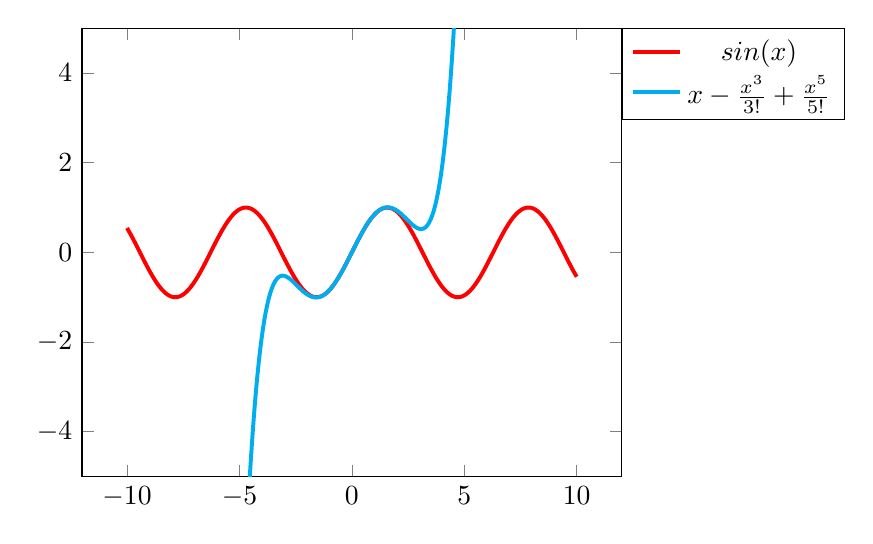
\begin{tikzpicture}
\begin{axis}[legend style={at={(1,1)},anchor=north west},ymin=-5, ymax=5]
\addplot[line width=0.5mm,color=red, domain=-10:10, samples=500]{sin(deg(x))};
\addlegendentry{\(sin(x)\)}
%\addplot[color=blue, domain=-10:10, samples=500]{x};
%\addlegendentry{\(x\)}
%\addplot[color=green, domain=-10:10, samples=500]{x-((x^3)/(3!))};
%\addlegendentry{\(x-\frac{x^3}{3!}\)}
\addplot[line width=0.5mm,color=cyan, domain=-5:5, samples=500]{x-((x^3)/(3!))+((x^5)/(5!))};
\addlegendentry{\(x-\frac{x^3}{3!}+\frac{x^5}{5!}\)}
%\addplot[color=black, domain=-7:7, samples=500]{x-((x^3)/(3!))+((x^5)/(5!))-((x^7)/(7!))};
%\addlegendentry{\(\mathsmaller{{x-\frac{x^3}{3!}+\frac{x^5}{5!}-\frac{x^7}{7!}}}\)}
\end{axis}
\end{tikzpicture}

{ For a sick interactive version: \url{https://www.desmos.com/calculator/elb2sjyuhu}}
\end{frame}

\begin{frame}
\frametitle{Example Taylor series question}
{\scriptsize
Compute the Taylor series of the function $f(x)=\sin x$ centered around $x=0$.

------------------------------------------------------------------------------

\pause
Solution: let's compute some derivatives:
\[f^{(0)}(x)=f(x)=\sin x\quad\quad\quad\quad f^{(0)}(0)=0\]
\vspace*{-\baselineskip}\pause\[f^{(1)}(x)=\cos x\quad\quad\quad\quad f^{(1)}(0)=1\]
\vspace*{-\baselineskip}\pause\[f^{(2)}(x)=-\sin x\quad\quad\quad\quad f^{(2)}(0)=0\]
\vspace*{-\baselineskip}\pause\[f^{(3)}(x)=-\cos x\quad\quad\quad\quad f^{(3)}(0)=-1\]
\vspace*{-\baselineskip}\pause\[f^{(4)}(x)=\sin x\quad\quad\quad\quad f^{(4)}(0)=0\]
\vspace*{-\baselineskip}\pause\[f^{(5)}(x)=\cos x\quad\quad\quad\quad f^{(5)}(0)=1\]

\pause We see a pattern! These derivatives will infinitely repeat in a cycle of four. Using the formula for Taylor series and some ingenuity, we get
\pause\[f(x)=\sum_{n=0}^\infty \frac{f^{(n)}(a)}{n!}(x-a)^n=\sum_{n=0}^\infty \frac{f^{(n)}(0)}{n!}x^n=\pmb{\sum_{n=0}^\infty \frac{(-1)^{n}}{(2n+1)!}x^{2n+1}}\]
}
\end{frame}

\begin{frame}
\frametitle{Taylor polynomials}

We had already seen \[f(x)=\sum_{n=0}^\infty \frac{f^{(n)}(a)}{n!}(x-a)^n\] but this is an infinite sum.

\pause Very often, only the first few terms will suffice in order to get a precise approximation. When we take only the first few terms such that we have a polynomial of degree $n$, then this is the \textbf{$\pmb{n}^{\text{th}}$ degree Taylor polynomial}.

\pause For example, the 5th degree Taylor polynomial of $\sin x$ at 0 is \[ x-\frac{x^3}{3!}+\frac{x^5}{5!}\approx\sin x\].

\end{frame}